%% 
%% Copyright 2007, 2008, 2009 Elsevier Ltd
%% 
%% This file is part of the 'Elsarticle Bundle'.
%% ---------------------------------------------
%% 
%% It may be distributed under the conditions of the LaTeX Project Public
%% License, either version 1.2 of this license or (at your option) any
%% later version.  The latest version of this license is in
%%    http://www.latex-project.org/lppl.txt
%% and version 1.2 or later is part of all distributions of LaTeX
%% version 1999/12/01 or later.
%% 
%% The list of all files belonging to the 'Elsarticle Bundle' is
%% given in the file `manifest.txt'.
%% 

%% Template article for Elsevier's document class `elsarticle'
%% with numbered style bibliographic references
%% SP 2008/03/01

\documentclass[preprint,12pt]{elsarticle}

%% Use the option review to obtain double line spacing
%% \documentclass[authoryear,preprint,review,12pt]{elsarticle}

%% Use the options 1p,twocolumn; 3p; 3p,twocolumn; 5p; or 5p,twocolumn
%% for a journal layout:
%% \documentclass[final,1p,times]{elsarticle}
%% \documentclass[final,1p,times,twocolumn]{elsarticle}
%% \documentclass[final,3p,times]{elsarticle}
%% \documentclass[final,3p,times,twocolumn]{elsarticle}
%% \documentclass[final,5p,times]{elsarticle}
%% \documentclass[final,5p,times,twocolumn]{elsarticle}

%% For including figures, graphicx.sty has been loaded in
%% elsarticle.cls. If you prefer to use the old commands
%% please give \usepackage{epsfig}

%% The amssymb package provides various useful mathematical symbols
% https://groups.google.com/forum/#!topic/comp.text.tex/mgzSLY8zCa8
% \expandafter\let\csname binom\endcsname\relax
% \expandafter\let\csname endebinom\endcsname\relax

\usepackage{amsmath}
\usepackage{amssymb}
\usepackage{amstext}
%% The amsthm package provides extended theorem environments
%% \usepackage{amsthm}

%% The lineno packages adds line numbers. Start line numbering with
%% \begin{linenumbers}, end it with \end{linenumbers}. Or switch it on
%% for the whole article with \linenumbers.
%% \usepackage{lineno}
\newcommand{\abs}[1]     {\left|#1\right|}
\newcommand{\norm}[1]    {\lVert#1\rVert}

\newcommand{\real}[1]    {\mathbb{R}^{#1}}
\newcommand{\cmplx}[1]   {\mathbb{C}^{#1}}

\newcommand{\paren}[1]   { \left( #1 \right) }
\newcommand{\lst}[1]     { \lbrace #1 \rbrace }

\newcommand{\matrx}[2]   {\paren{\begin{array}{#1}#2\end{array}}}
%\newcommand{\binom}[2]   {\paren{\begin{array}{c} #1\\ #2 \end{array}}}

\newcommand{\disc}       { \overline{D}_{2} }

\newcommand{\floor}[1]   {\lfloor #1 \rfloor}
\newcommand{\ceiling}[1] {\lceil #1 \rceil}

\newcommand{\zr}[2]      { R_{#1}^{#2}\paren{r} }
\newcommand{\mst}[0]     {M\"untz-Sz\'asz }
\newcommand{\term}[0]    { \sqrt{1-2z\paren{1-2r^{2}}+z^{2}} }
\newcommand{\spn}[1]     {\text{sp\,} \lst{ #1 }}

\newcommand{\Or}[1]      { \mathcal{O}\paren{#1} }

% theorems and such
\newtheorem{myDefinition}{Definition}
\newtheorem{myTheorem}{Theorem}
\newtheorem{myLemma}{Lemma}

\endinput

\journal{Advances in Mathematics}

\begin{document}

\begin{frontmatter}

%% Title, authors and addresses

%% use the tnoteqref command within \title for footnotes;
%% use the tnotetext command for theassociated footnote;
%% use the fnref command within \author or \address for footnotes;
%% use the fntext command for theassociated footnote;
%% use the corref command within \author for corresponding author footnotes;
%% use the cortext command for theassociated footnote;
%% use the ead command for the email address,
%% and the form \ead[url] for the home page:
%% \title{Title\tnoteqref{label1}}
%% \tnotetext[label1]{}
%% \author{Name\corref{cor1}\fnref{label2}}
%% \ead{email address}
%% \ead[url]{home page}
%% \fntext[label2]{}
%% \cortext[cor1]{}
%% \address{Address\fnref{label3}}
%% \fntext[label3]{}

\title{Surprising homotopies in the Zernike basis}

%% use optional labels to link authors explicitly to addresses:
%% \author[label1,label2]{}
%% \address[label1]{}
%% \address[label2]{}

\author[1,2,3]{D. M. Topa\corref{cor1}}
\ead{dantopa@unm.edu}
\author[1]    {J. H. Cooley}
\ead{jhcooley@lanl.gov}
\author[2]    {P. F. Embid}
\ead{pfembid@math.unm.edu}

\address[1]{Los Alamos National Laboratory, Los Alamos, NM USA}
\address[2]{Department of Mathematics and Statistics, \\University of New Mexico, Albuquerque, NM USA}
\address[3]{Engility Corporation, \\USACE Engineer Research and Development Center, Vicksburg, NM USA}

\cortext[cor1]{Corresponding author}

\begin{abstract}
The smoothness of a function in physical space is related to the decay of the Fourier coefficients in wavenumber space. We generalize this idea to the Fourier-like polynomial basis of Zernike and present families of functions which have equivalent smoothness or regularity in the Zernike basis. Such equivalence connects the wavefronts for static and inertial point sources and leads to new classes of surfaces, the ultra--cone and the ultra--sphere.
\end{abstract}

\begin{keyword}
%% keywords here, in the form: keyword \sep keyword
Homotopy \sep Zernike polynomials \sep polynomial approximation \sep ultra surfaces \sep regularity \sep wavefronts
%% PACS codes here, in the form: \PACS code \sep code
\PACS 02.30.Gp \sep 02.30.Mv \sep 07.60.-j
%% MSC codes here, in the form: \MSC code \sep code
%% or \MSC[2008] code \sep code (2000 is the default)
\MSC[2010] 42C10 \sep 78-04
\end{keyword}

\end{frontmatter}

%% \linenumbers

%% main text
\section{Introduction}
\label{sec:introduction}
The prototypical wavefront surfaces for point sources in the field of optics are the cone and the sphere. The sphere 
% = =  e q u a t i o n
  \begin{equation}
    %\begin{split}
      B(r) = \sqrt{1-r^{2}}
    %\end{split}
    \label{eq:sphere}
  \end{equation}
% = =
represents the surface of constant phase for a \emph{static} point source \cite[\S1.3.2]{BW}, \cite[\S2.9]{Hecht}, \cite[p. 33]{do}, the cone 
% = =  e q u a t i o n
  \begin{equation}
    %\begin{split}
      A(r) = 1 - r
    %\end{split}
    \label{eq:cone}
  \end{equation}
% = =
an \emph{inertial} point source \cite[p. 146]{do}, \cite[p. 122]{Longair}, \cite[ch. 3]{Green}. These surfaces (shown in figure \ref{fig:wavefronts}) manifest different behavior in their derivatives: the cone lacks a tangent at the vertex, whereas the sphere exhibits a vertical tangent at its edge. So it comes as a surprise that when one computes the expansion coefficients for the cone and the sphere in the Zernike polynomials that they have exactly the same decay \cite{22358}. The terms for $n=0,2,4,\dots,12$ are
% = =  e q u a t i o n
  \begin{equation}
    \begin{split}
      a_{n} &= \paren{ \frac{1}{3},-\frac{2}{5},\phantom{-}\frac{2}{21},-\frac{2}{45},\phantom{-}\frac{2}{77},-\frac{2}{117},\phantom{-}\frac{2}{165}, \dots }, \\
      b_{n} &= \paren{ \frac{2}{3},-\frac{2}{5},-\frac{2}{21},-\frac{2}{45},-\frac{2}{77},-\frac{2}{117},-\frac{2}{165}, \dots }. \\
    \end{split}
    \label{eqn:archeoamps}
  \end{equation}
% = =
If $a_{2k}$ are the coefficients in the Zernike polynomial basis for the cone and $b_{2k}$ for the sphere then
\begin{equation}
  a_{2k} = \paren{-1}^{k+1} b_{2k}, \quad n = 2, 4, 6, \dots
\end{equation}
hence $\abs{a_{2k}} = \abs{b_{2k}}$. In this paper we want to explain this fact and explore whether there are other families of surfaces exhibiting a similar behavior.

%
%   \includegraphics[ trim = 0cm 0cm 0cm 1cm, width = 2.5in ]{eps/sphere} \qquad
\begin{figure}[t] %  figure placement: here, top, bottom, or page
   \centering
%   \includegraphics[ width = 2.5in ]{graphics/sphere} \qquad
%   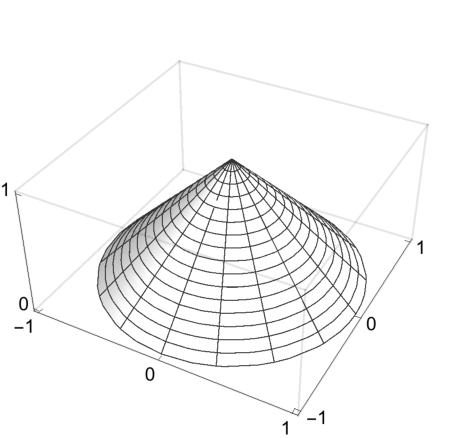
\includegraphics[ width = 2.5in ]{graphics/cone} 
   \includegraphics[ width = 2.5in ]{graphics/sphere} \qquad
   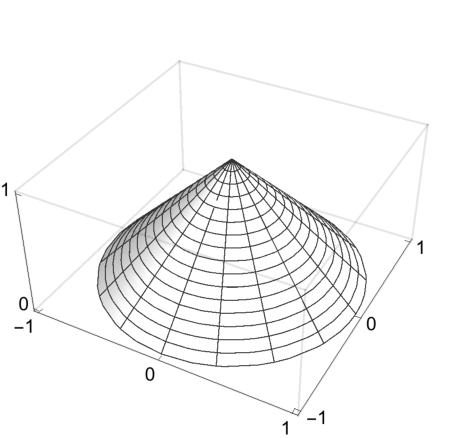
\includegraphics[ width = 2.5in ]{graphics/cone} 
   \caption{Two fundamental wavefronts: the sphere (left) and the cone (right). The sphere represents the wavefront created by a static point charge, the cone an inertial point charge (Cherenkov radiation).}
   \label{fig:wavefronts}
\end{figure}
%

%   +   +   +   +   +   +   +   +   +   +   +   +   +   +   +   +   +   +   +   +   +   +   +   +   +   +   +   +   +   +
%\section{Methods}
%\label{sec:methods}

%   +   +   +   +   +   +   +   +   +   +   +   +   +   +   +   +   +   +   +   +   +   +   +   +   +   +   +   +   +   +
\section{Theory and methods}
\label{sec:theory}
%   ++   ++   ++   ++   ++   ++   ++   ++   ++   ++   ++   ++   ++   ++   ++   ++   ++   ++   ++   ++   ++   ++   ++   ++ 
\subsection{Regularity}
In the theory of Fourier series, it is a well established fact (e.g. \cite[example 2.4.9]{classic}, \cite[ch. 6]{modern}) that there is a correlation between the smoothness of a $2\pi-$periodic function $f(x)$ in physical space and the decay of the associated Fourier coefficients $c_{n}$, where
\begin{equation}
  f(x) = \sum_{n=-\infty}^{\infty} c_{n} e^{inx}\ .
\end{equation}
In fact, if $f(x)$ and its derivatives $f^{(k)}(x)$, $k=1,2,\dots,p$ are continuous then $c_{n} = \Or{n^{-p}}$ as $n\to\infty$. Conversely, if $c_{n} = \Or{n^{-p}}$ as $n\to\infty$, one can guarantee that $f^{(k)}(x)$ is continuous for $k=1,2,\dots,p-2$ by the Weierstrass M-test (because the coefficients of $f^{(k)}(x)$ are $c_{n}^{(k)} = \paren{in}^{k} c_{n}$, hence $c_{n}^{(k)} = \Or{n^{-p+k}}$ and $\sum \frac{1}{n^{p-k}} \le \sum \frac{1}{n^{2}} < \infty$). Moreover this relation between smoothness in physical space and decay of the Fourier amplitudes is so fundamental in mathematics that it gave rise to the so-called Sobolev spaces, where the smoothness of the function $f(x)$ is understood in terms of the $L^{2}-$norm and corresponding decay of the coefficients is given in the related $l^{2}-$norm via the Parseval identity
\begin{equation}
  \int_{-\pi}^{\pi} \abs{\frac{d^{k}f}{dx^{k}}}^{2} dx = \sum_{n=-\infty}^{n=\infty} n^{2k} \abs{c_{n}}^{2} \ .
\end{equation}
Similar statements hold true to a degree for other orthogonal families of functions like the Legendre polynomials or the Zernike polynomials.

%   ++   ++   ++   ++   ++   ++   ++   ++   ++   ++   ++   ++   ++   ++   ++   ++   ++   ++   ++   ++   ++   ++   ++   ++ 
\subsection{Equality and equivalence}
Because of the connection between smoothness in space and decay of the Fourier coefficients mentioned above we want to study the regularity properties of functions in physical space by comparing the behavior of the Fourier coefficients. To this end we introduce the following concepts.
Consider two functions $A(r)$ and $B(r)$ continuous on the interval $0\le r\le 1$ and their respective Fourier-Zernike representations:
\begin{equation}
  \begin{split}
    A(r) & = \sum_{k=0}^{\infty} a_{2k} Z_{2k}^{0}(r), \\
    B(r) & = \sum_{k=0}^{\infty} b_{2k} Z_{2k}^{0}(r).
  \end{split}
\end{equation}
We shall see that the class of Zernike polynomials with angular frequency $m=0$ are a complete set of rotationally invariant polynomials.
The amplitudes are computed using a projection operator. For example,
\begin{equation}
  a_{2k} = \frac{\int_{0}^{1}{A(r) Z_{2k}^{0}(r)rdr}} {\int_{0}^{1}{\paren{Z_{2k}^{0}}^{2}(r)rdr}}.
\end{equation}

From the completeness of the Zernike polynomials in $L^{2}[0,1]$ (with weight $r$) we know that the two functions are equal\footnote{Almost everywhere since convergence is in the $L^{2}$ sense in general.} iff they have the same coefficients:
\begin{equation}
  A(r) = B(r) \quad \text{if and only if} \quad a_{2k} = b_{2k}, \quad \ k=0,1,2,\dots
\end{equation}
We say that two functions are equivalent iff the corresponding Fourier-Zernike coefficients have the same asymptotic behavior, that is:
\begin{equation}
  A(r) \equiv B(r) \quad \text{if and only if} \quad \lim_{k\to\infty} \abs{\frac{a_{2k}}{b_{2k}}} = c \ne 0, \quad \ k=1,2,\dots
  \label{asymptote}
\end{equation}
It is not difficult to check that this is an equivalence relation. Certainly if $A(r)=B(r)$ then $A(r) \equiv B(r)$. Also, if $\abs{a_{2k}} = \abs{b_{2k}}$ for all $n$ then $A(r) \equiv B(r)$. This notion of equivalence is clearly motivated by the fact that the asymptotic decay of the Fourier coefficients affects the regularity of the function.

Moreover, since this notion of equivalence is an asymptotic one, it is not changed by the addition of a constant, or more generally any polynomial. That is, if
\begin{equation}
  B(r) = A(r) + p(r)
\end{equation}
where $p(r)$ is any polynomial then $B(r) \equiv A(r)$ (assuming there is a finite number of nonzero Fourier coefficients of $p(r)$).

%   ++   ++   ++   ++   ++   ++   ++   ++   ++   ++   ++   ++   ++   ++   ++   ++   ++   ++   ++   ++   ++   ++   ++   ++ 
\subsection{The disk polynomials of Zernike}
Because of the nature of our measurement systems, we are concerned with expansions over the closed unit disk, $\overline{D}_{2} = \lst{\paren{r,\phi}\colon 0\le r\le 1, 0\le \phi < 2\pi}$. The need for a complete orthogonal set of basis functions for this domain leads immediately to the disk\footnote{Zernike called his set the circle polynomials. However, there is a need to distinguish his set which is orthogonal over the unit disk from those orthogonal over the unit circle. See for example Simon \cite{Simon}. The Zernike polynomials are related to the Kanjin \cite{Kanjin} disk polynomials by exact affine transformations.} polynomials of Zernike \cite{Zernike}. These functions are indexed by an order $n=0,1,2,\dots$ and an angular frequency $m=-n, -n+2,\cdots,n-2,n$ such that the difference $n-m$ is always a non-negative, even number.

Zernike's set was originally posited as a Fourier sine series with polynomial weighting. To quote\footnote{The mathematical notation has been altered slightly to match current practice.} from his paper
%
\begin{quotation}
  Expressed in terms of $r$ and $\phi$, these \emph{circle polynomials} were found to have the form $R_{n}^{m}(r) \sin m\paren{\phi - a}$ where $n-m$ is even, $m\le n$, and $R$ is a finite hypergeometric series (Jacobi polynomial):
\end{quotation}
%
\begin{equation}
  \begin{split}
    R_{n}^{m}(r) 
    & = \paren{-1}^{\frac{n-m}{2}} \tbinom{\frac{n-m}{2}}{m} r^{m}\,_{2}F_{1} \paren{\frac{n+m+2}{2}, -\frac{n-m}{2}, m+1,r^{2}}\\
%    & = \paren{-1}^{\frac{n-m}{2}} \choose{\frac{n-m}{2}}{m} r^{m}\,_{2}F_{1} \paren{\frac{n+m+2}{2}, -\frac{n-m}{2}, m+1,r^{2}}\\
    & = \frac{r^{-m}}{\paren{\frac{n-m}{2}}!} \paren{\frac{d}{d\paren{r^{2}}}}^{\frac{n-m}{2}} \left\{r^{n+m} \paren{r^{2}-1}^{\frac{n-m}{2}} \right\}
  \end{split}
\end{equation}

Wolf and his collaborators Bhatia \cite{Wolf} and Born \cite{BW} emphasize a natural way to think of these polynomials is as elements in a Fourier-like expansion. We can describe an arbitrary continuous function $\psi\paren{r, \phi}\in C(\disc)$ as a uniformly convergent decomposition of Zernike polynomials
\begin{equation}
  \psi\paren{r, \phi} = \sum_{n=0}^{\infty}\sum_{m=-n}^{n(2)} \alpha_{k} R_{n}^{m}(r) e^{i m \phi}, \quad \alpha\in\cmplx{} .
\end{equation}
The superscript on the $m$ summation indicates that the increment on the $m$ variable is 2: $m = -n, -n+2, \dots, n-2, 2$.

The generating function for the radial polynomials is given as \cite[p. 525]{BW}
\begin{equation}
  \frac{\paren{1+z-\term}^{m}} {\paren{2zr}^{m} \term} = \sum_{s=0}^{\infty} z^{s} R_{m+2s}^{\pm m}(r)
  \label{eq:zernikegen}
\end{equation}
This initial investigation is concerned only with the rotationally invariant polynomials which are characterized by $m=0$. The recursion relationship for this reduced set is
%%%
\begin{equation}
  R_{2k}^{0}(r) = \sum_{j=0}^{k}{\paren{-1}^j\frac{(2k-j)!}{j!\paren{\paren{k-j}!}^{2}}r^{2(k-j)}} .
  \label{eq:reduced}
\end{equation}
%%%
The first few terms of this sequence are shown here:
\begin{multline}
\left\{ R_{0}^{0}(r),  R_{2}^{0}(r),  R_{4}^{0}(r),  R_{6}^{0}(r), \dots \right\} = \\
  \left\{1, 2r^2-1, 6r^4-6 r^2+1, 20r^6-30 r^4 + 12 r^2-1, \dots \right\}.
\end{multline}
This is just a Gram-Schmidt orthogonalization of radial polynomials of even order $\{1,r^{2},r^{4},\dots\}$ over the domain $0\le r\le1$ with monic normalization $R_{n}^{m}(1)=1$.\footnote{Here $n=0,1,2,\dots$ and $m$ is constrained such that $n-m$ must be even.} The Weierstrass approximation theorem guarantees that polynomials are dense in the space of continuous functions.\footnote{Using the uniform norm.} The polynomials of interest, the span $\lst{r^{2k}}_{k=0}^{\infty}$, have integer powers and we appeal to the \mst theorem \cite[p. 88]{Lax},\footnote{See also Siegal's \cite{Siegal} proofs.} which asserts that the span of the monomials $\lst{r^{j_{m}}}_{m=0}^{\infty}$ is dense in the space of continuous functions if and only if $\sum_{m=0}^{\infty}\frac{1}{j_{m}} = \infty$.
%
The family of functions $R_{n}^{0}(r)$ can be generated by a Gram-Schmidt orthogonalization of the sequence of the even polynomial powers $\lst{1,r^{2},r^{4},\dots} = \lst{r^{2k}}_{n=0}^{\infty}$ and therefore the two spans are equal:
  % % % EQUATION
  \begin{equation}
    \text{span } \lst{r^{2k}}_{k=0}^{\infty} = \text{span } \lst{R_{2k}^{0}}_{k=0}^{\infty}
  \end{equation}
  % % %
By the extension of the \mst theorem to the unit disk \cite{ms} we can cite the fact that $\sum_{k=1}^{\infty}\frac{1}{2k} = \infty$ signals the culled set of disk polynomials of Zernike $\lst{R_{2k}^{0}}_{k=0}^{\infty}$ are dense in the space of rotationally invariant functions over the unit disk which guarantees uniform convergence of the sequence of partial sums.

The normalization for the set with zero angular velocity is given by
% = =  e q u a t i o n
  \begin{equation}
    %\begin{split}
      \int_{\disc} \paren{R_{2k}^{0}(r)}^{2} r dr d\phi = \frac{1} { 2\paren{2k + 1} }, \qquad k = 0, 1, 2, \dots
    %\end{split}
    %\label{eqn:}
  \end{equation}
% = =

%   ++   ++   ++   ++   ++   ++   ++   ++   ++   ++   ++   ++   ++   ++   ++   ++   ++   ++   ++   ++   ++   ++   ++   ++ 
\subsection{Expansions for the sphere and the cone}
The Zernike coefficients for the cone and the sphere can be computed in a straightforward, albeit not illuminating way, by the identities
\begin{equation}
    \begin{split}
          \int_{0}^{1} \paren{\paren{1-r}r^{n}}rdr 
      &= \frac{1}{\paren{n+2}\paren{n+3}}, \\
    \int_{0}^{1} \paren{\sqrt{1-r^{2}} r^{n}}rdr 
%      &= \frac{\sqrt{\pi}}{4} \frac{\Gamma{\paren{\frac{n+2}{n}}}} {\Gamma{\paren{\frac{n+5}{n}}}}.
      &= \frac{\sqrt{\pi}}{4} \Gamma{\paren{\frac{n+2}{n}}}  \paren{\Gamma{\paren{\frac{n+5}{n}}}}^{-1},
    \end{split}
    \label{eq:monomial}
\end{equation}
with $n$ being positive and even. These relations yield the explicit series expansions for the cone, $A(r)$, the sphere, $B(r)$, as
% = =  e q u a t i o n
  \begin{equation}
    \begin{split}
      A(r) &= \frac{1}{3} - \sum_{k=1}^{\infty} \frac{2\paren{-1}^{k+1}}{\paren{2k-1} \paren{2k+3}} Z_{2k}^{0}(r),\\
      B(r) &= \frac{2}{3} - \sum_{k=1}^{\infty} \frac{2}{\paren{2k-1} \paren{2k+3}} Z_{2k}^{0}(r).
    \end{split}
    %\label{eqn:}
  \end{equation}
% = =
It is apparent from the above expansions that the coefficients
\begin{equation}
  A_{2k} = \paren{-1}^{k+1}B_{2k}, \quad k=1,2,\dots
\end{equation}
and therefore
\begin{equation}
  A(r) \equiv B(r) \quad \paren{\lim_{k\to\infty} \frac{\abs{A_{2k}}} {\abs{B_{2k}}} = 1}.
\end{equation}
This paper examines the equivalence and extends this concept by generalizing definitions of these two surfaces.

%   +   +   +   +   +   +   +   +   +   +   +   +   +   +   +   +   +   +   +   +   +   +   +   +   +   +   +   +   +   +
\section{Results}
\label{sec:results}
%   ++   ++   ++   ++   ++   ++   ++   ++   ++   ++   ++   ++   ++   ++   ++   ++   ++   ++   ++   ++   ++   ++   ++   ++ 
\subsection{Relationship between the coefficients for the sphere and the cone}
Here we establish the simple yet surprising fact that the coefficients of the cone and the sphere are related by the formulas
% = =  e q u a t i o n
  \begin{equation}
    \begin{split}
      A_{0} &= 1 - B_{0}, \\
      A_{2k} &= \paren{-1}^{k+1}B_{2k}, \quad k=1,2,\dots
    \end{split}
    \label{eq:23}
  \end{equation}
% = =
This is a consequence of two facts. First, the radial Zernike polynomials $\paren{m=0}$ are nothing more than the Legendre polynomials in the variable $\rho=2r^{2}-1$. Indeed, if we set $m=0$ in \eqref{eq:zernikegen} we get
\begin{equation}
%  \frac{1} {\term} = \sum_{s=0}^{\infty} z^{s} R_{2s}^{0}(r).
  \paren{\term}^{-1/2} = \sum_{s=0}^{\infty} z^{s} R_{2s}^{0}(r).
\end{equation}
which is nothing more than the generating function for the Legendre polynomials
\begin{equation}
%  \frac{1} {\sqrt{1-2z\rho+z^{2}}} = \sum_{s=0}^{\infty} z^{s}P_{s}(\rho).
  \paren{\sqrt{1-2z\rho+z^{2}}}^{-1/2} = \sum_{s=0}^{\infty} z^{s}P_{s}(\rho).
\end{equation}
after the identification $\rho=2r^{2}-1$, $\paren{-1\le \rho \le 1,\ 0 \le r \le 1}$. That is, if $\rho=2r^{2}-1$ then 
\begin{equation}
  R_{2k}^{0}(r) = P_{k}\paren{2r^{2}-1} = P_{k}\paren{\rho}.
\end{equation}
Second, in the variable $\rho$ the sphere and the cone become
% = =  e q u a t i o n
  \begin{equation}
    \begin{split}
    %
      A\paren{\rho} & = 1 - \sqrt{\frac{1+\rho}{2}} = 1 + \alpha\paren{\rho}, \\
    %
      B\paren{\rho} & = \sqrt{\frac{1-\rho}{2}} = \beta\paren{\rho}.
    %
    \end{split}
    \label{eq:rhov}
  \end{equation}
% = =
The key observation is that the coefficients obey the parity relation
\begin{equation}
  \alpha\paren{\rho} = -\beta\paren{-\rho}.
  \label{eq:parity}
\end{equation}
In terms of the new variable the expansion coefficients take the form
% = =  e q u a t i o n
  \begin{equation}
    \begin{split}
    \alpha\paren{\rho} & = \sum_{k=0}^{\infty} \alpha_{k} P_{k}\paren{\rho}, 
     \quad \alpha_{k} = \frac{\int_{-1}^{1}\alpha(\rho) P_{k}\paren{\rho} d\rho}{\int_{-1}^{1} P_{k}^{2}\paren{\rho} d\rho} \\
%
    \beta\paren{\rho} & = \sum_{k=0}^{\infty} \beta_{k} P_{k}\paren{\rho}, 
     \quad \beta_{k} = \frac{\int_{-1}^{1}\beta(\rho) P_{k}\paren{\rho} d\rho}{\int_{-1}^{1} P_{k}^{2}\paren{\rho} d\rho}.
    %
    \end{split}
    \label{eq:defn}
  \end{equation}
% = =
The parity of the Legendre functions matches the parity of the index:
\begin{equation}
  P_{k}\paren{\rho} = \paren{-1}^{k} P_{k}\paren{-\rho}
\end{equation}
and this explains the oscillation in the sign exhibited in \eqref{eq:23}:
\begin{equation}
  \alpha_{2k} = \paren{-1}^{k+1} \beta_{2k}.
  \label{eq:equals}
\end{equation}
In terms of smoothness it clearly follows that
\begin{equation}
  \abs{\alpha_{2k}} = \abs{\beta_{2k}},\ k=1,2,\dots,
  \label{eq:canona}
\end{equation}
and the zero order (average) terms satisfy
\begin{equation}
  a_{0} + b_{0} = \alpha_{0} + \beta_{0} = 1.
  \label{eq:canonb}
\end{equation}
For the case of the cone and the sphere we see from \eqref{eq:defn} that 
\begin{equation}
  a_{0} = \frac{1}{3}, \quad
  b_{0} = \frac{2}{3}.
\end{equation}

The equivalence of regularity for these two different surfaces stemmed from two facts. First is the behavior of the first derivative. Neither function is differentiable over the domain of the unit disk. The derivative of the cone has a jump discontinuity at the apex, yet the function satisfies the Lipschitz condition in any neighborhood of the origin. The derivative of the sphere diverges at the boundary, yet the function is of bounded variation. Second is the choice of the Zernike basis. Inspection of \eqref{eq:monomial} establishes the amplitudes do not have equal magnitudes in the monomial basis. 

Surprised to find the homotopy between these very different surfaces, we searched for other cases. Only one line of investigation bore fruit: moving the pathologies to higher derivatives.

%   ++   ++   ++   ++   ++   ++   ++   ++   ++   ++   ++   ++   ++   ++   ++   ++   ++   ++   ++   ++   ++   ++   ++   ++ 
\subsection{Ultra--cone and ultra--sphere}
Using the results from the previous section, one can generalize the expression for these two surfaces. Such an extension leads to the definition of the ultra--cone family
\begin{equation}
  A(\mu,r) = 1-r^{\mu}, \quad 0<\mu<\infty
  \label{eq:mu:cone}
\end{equation}
and the ultra--sphere family
\begin{equation}
  B(\mu,r) = \paren{\sqrt{1-r^{2}}}^{\mu}, \quad 0<\mu<\infty.
  \label{eq:mu:sphere}
\end{equation}
How do the ultra--surfaces change as $\mu$ increases and decreases? To answer this question two sequences are evaluated; an arithmetically increasing sequence $\mu={1,3,5,7,9}$, and a geometrically decreasing sequence $\mu={1,2^{-1},2^{-2},2^{-3},2^{-5}}$. Behavior of the amplitudes $a_{n}(\mu)$ are shown in figures \ref{fig:mu big} and \ref{fig:mu small}. The figures reveal the matryoshka behavior of the graphs. For the ultra--sphere with $\mu\ge1$, the graphs for increasing $\mu$ nest inside the graphs of lower $\mu$. When $\mu \le1$ the graphs of smaller $\mu$ nest inside those of larger $\mu$. For the ultra--cone these nesting patterns are reversed.

%%%%%                                                                         table 1
\begin{table}[htbp]
\begin{center}
\begin{tabular}{ccc}
%
 ultra--cone & \qquad & ultra--sphere \\
 $\mu = 1, 3, 5, 7, 9$ && $\mu = 1, 3, 5, 7, 9$ \\[10pt]
%
   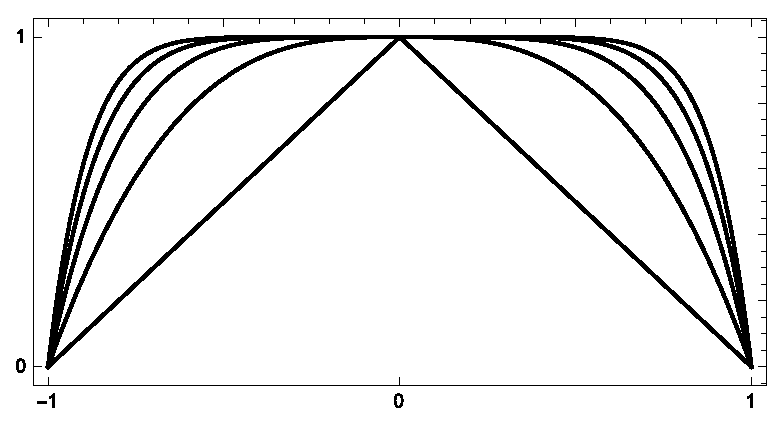
\includegraphics[ width = 2.5in ]{graphics/cone_increase}
&& 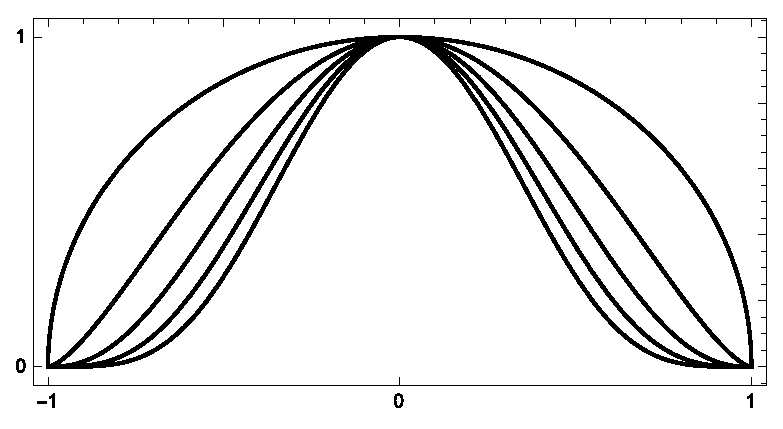
\includegraphics[ width = 2.5in ]{graphics/sphere_increase} \\
%
\end{tabular}
\end{center}
\caption{The sequence of equivalence for the ultra--cone (left) and the ultra--sphere (right) with $\mu$ an increasing sequence of odd integers. For these cases the discontinuities are moving to higher derivatives in lock step. The ultra--cone has at $r=0$ a jump in the $\mu$th derivative. The ultra--sphere has at $r=\pm1$ unbounded growth in the $\mu$th derivative. The ultra--cones envelope greater and greater area while the ultra--spheres envelope less and less.}
\label{tab:increase}
\end{table}%

%%%%%                                                                         table 2
\begin{table}[htbp]
\begin{center}
\begin{tabular}{ccc}
%
 ultra--cone & \qquad & ultra--sphere \\
 $\mu = 1, 2^{-1}, 2^{-2}, 2^{-3}, 2^{-4}$ && $\mu = 1, 2^{-1}, 2^{-2}, 2^{-3}, 2^{-4}$ \\[10pt]
%
   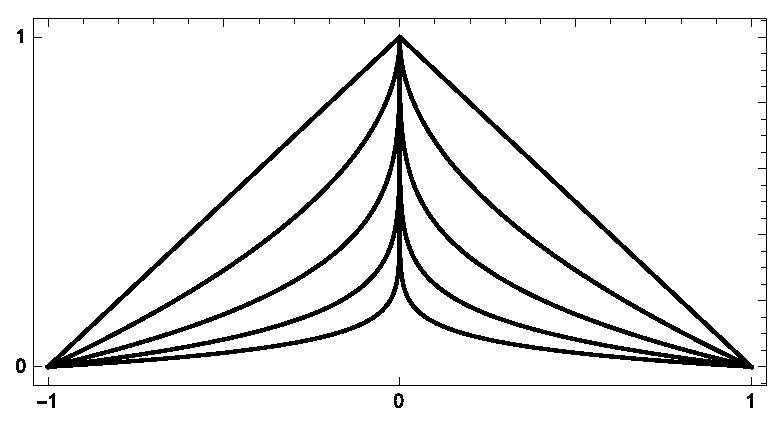
\includegraphics[ width = 2.5in ]{graphics/cone_decrease}
&& 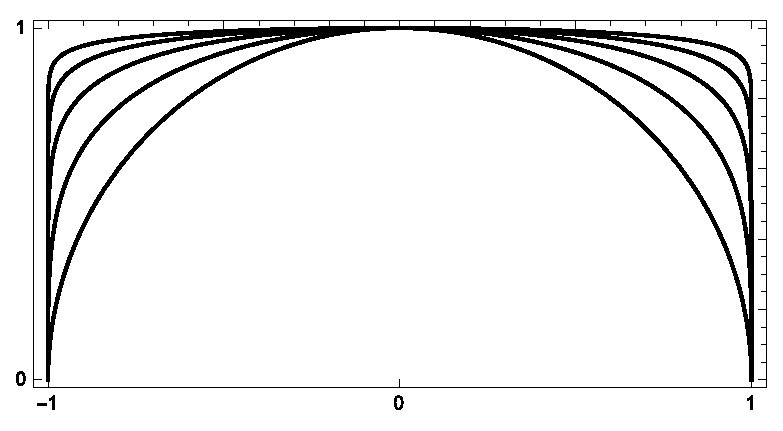
\includegraphics[ width = 2.5in ]{graphics/sphere_decrease} \\
%
\end{tabular}
\end{center}
\caption{The sequence of equivalence for the ultra--cone (left) and the ultra--sphere (right) with $\mu$ a decreasing geometric series. For the ultra--cone the first derivative is not defined at the origin. For the ultra--sphere the first-derivative is unbounded at the boundary.}
\label{tab:decrease}
\end{table}
%%%

The figures in tables \ref{tab:increase} and \ref{tab:decrease} are helpful for comparing changes within a homotopy family within a $\mu$ sequence. The figures in table \ref{tab:progression} help to relate the two families across the full spectrum of $\mu$. 
%%%%%                                                                         table 3
\begin{table}[htbp]
\caption{Function sequences for the ultra--sphere and the ultra--cone showing values for the parameter $\mu$ in \eqref{eq:mu:cone} and \eqref{eq:mu:sphere}. For $\mu\le 1$ the pathologies in the first derivative persist (on the boundary for the ultra--cone, at the origin for the ultra--sphere). When $\mu\ge 1$ the pathologies appear only for the odd integers. When $\mu=1$ we recover the sphere and the cone of equations \eqref{eq:sphere} and  \eqref{eq:cone}. The special value of $\mu = 2$ is  where the two ultra surfaces are the same, i.e. $A(2,r) = B(2,r)$.}
	\begin{center}
		\begin{tabular}{ccccc}
		  %
		   $\mu$ && ultra--sphere && ultra--cone \\\hline
%		  %
%		   $\frac{1}{4}$ & \qquad \qquad & 
% 		   \raisebox{-0.5\height}{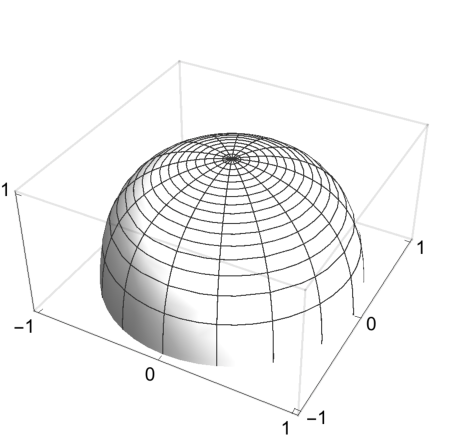
\includegraphics [ width = 1.25in ] {graphics/usphere_025}} & \qquad \qquad &
%		   \raisebox{-0.5\height}{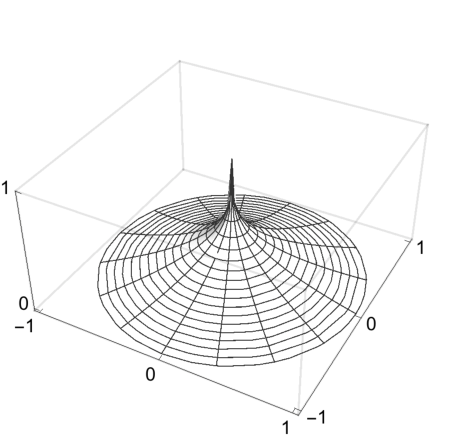
\includegraphics [ width = 1.25in ] {graphics/ucone_025}}   \\
%		  %
%		   $\frac{1}{2}$ && 
%		   \raisebox{-0.5\height}{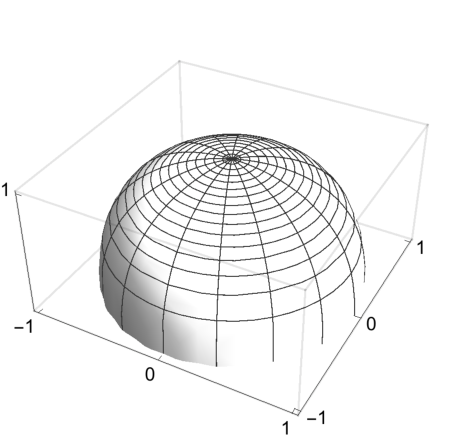
\includegraphics [ width = 1.25in ] {graphics/usphere_05}} &&
%		   \raisebox{-0.5\height}{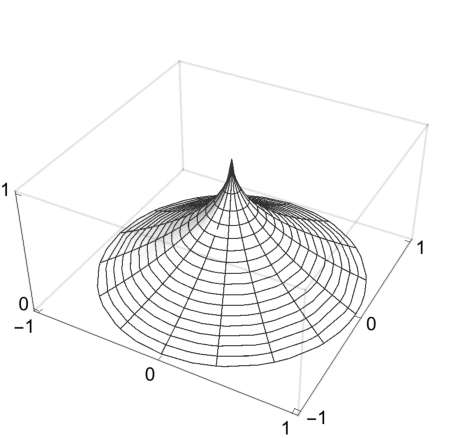
\includegraphics [ width = 1.25in ] {graphics/ucone_05}}   \\
%		  %
%		   $1$ && 
%		   \raisebox{-0.5\height}{\includegraphics [ width = 1.25in ] {graphics/sphere}} &&
%		   \raisebox{-0.5\height}{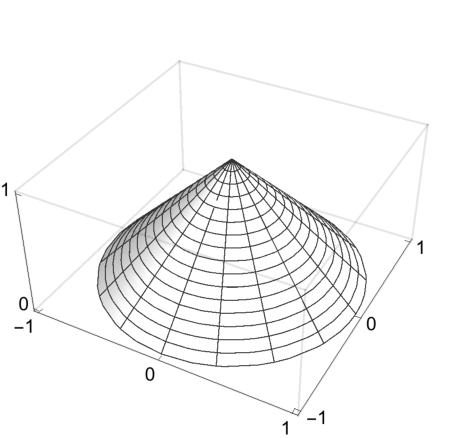
\includegraphics [ width = 1.25in ] {graphics/cone}}   \\
%		  %
%		   $2$ && 
%		   \raisebox{-0.5\height}{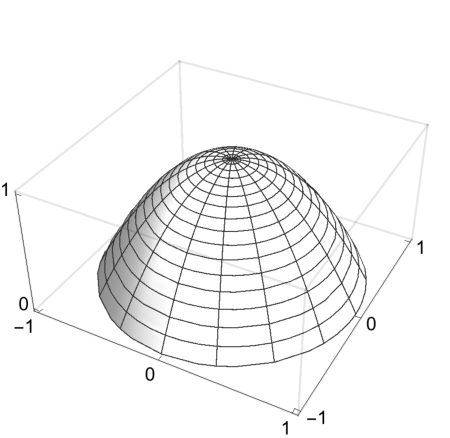
\includegraphics [ width = 1.25in ] {graphics/usphere_2}} &&
%		   \raisebox{-0.5\height}{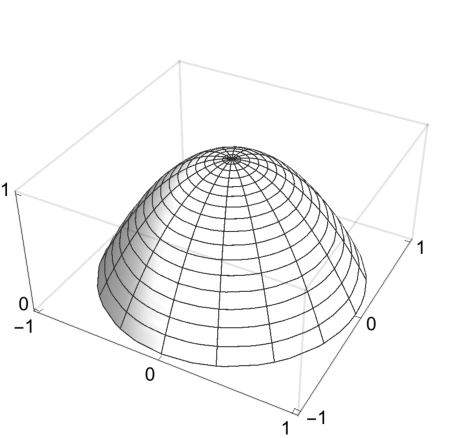
\includegraphics [ width = 1.25in ] {graphics/ucone_2}}   \\
%		  %
%		   $3$ && 
%			 \raisebox{-0.5\height}{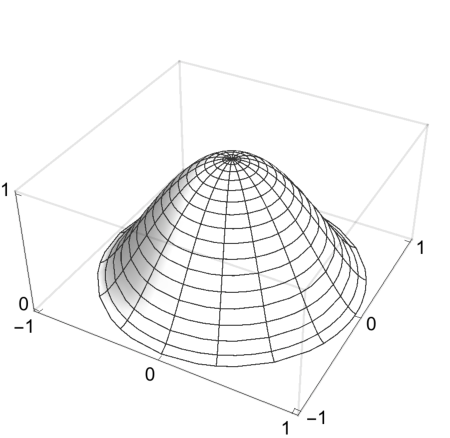
\includegraphics [ width = 1.25in ] {graphics/usphere_3}} &&
%		   \raisebox{-0.5\height}{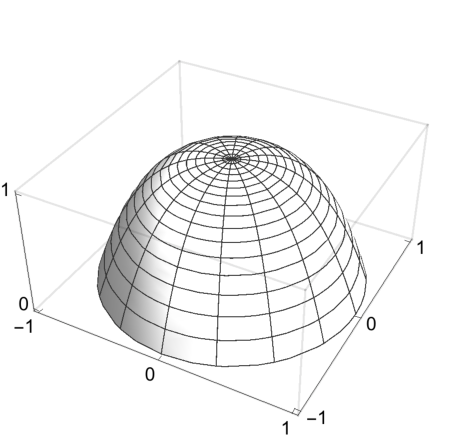
\includegraphics [ width = 1.25in ] {graphics/ucone_3}}   
		  %
		   $\frac{1}{4}$ & \qquad \qquad & 
 		   \raisebox{-0.5\height}{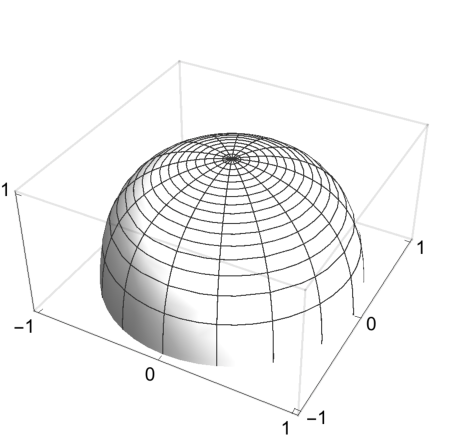
\includegraphics [ width = 1.25in ] {graphics/usphere_025}} & \qquad \qquad &
		   \raisebox{-0.5\height}{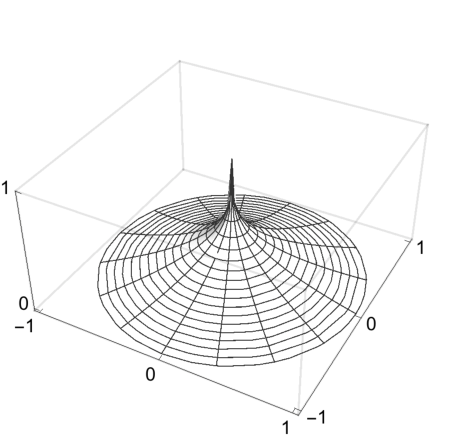
\includegraphics [ width = 1.25in ] {graphics/ucone_025}}   \\
		  %
		   $\frac{1}{2}$ && 
		   \raisebox{-0.5\height}{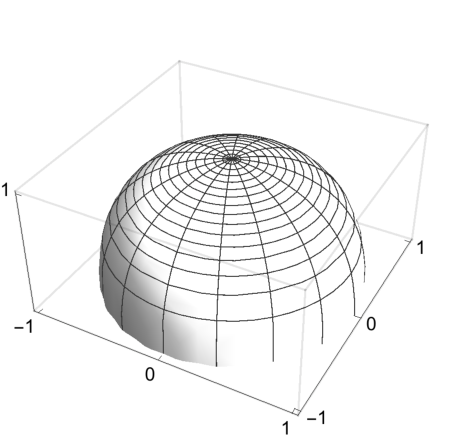
\includegraphics [ width = 1.25in ] {graphics/usphere_05}} &&
		   \raisebox{-0.5\height}{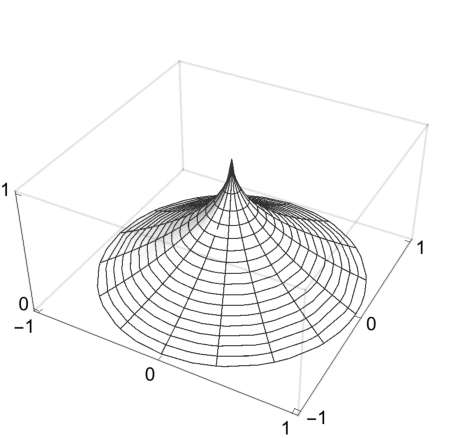
\includegraphics [ width = 1.25in ] {graphics/ucone_05}}   \\
		  %
		   $1$ && 
		   \raisebox{-0.5\height}{\includegraphics [ width = 1.25in ] {graphics/sphere}} &&
		   \raisebox{-0.5\height}{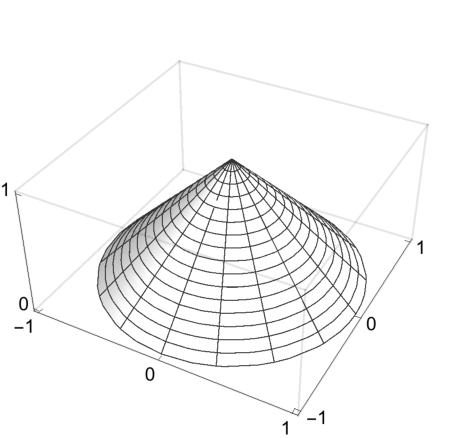
\includegraphics [ width = 1.25in ] {graphics/cone}}   \\
		  %
		   $2$ && 
		   \raisebox{-0.5\height}{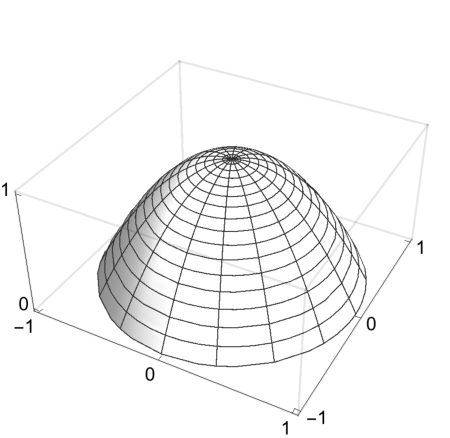
\includegraphics [ width = 1.25in ] {graphics/usphere_2}} &&
		   \raisebox{-0.5\height}{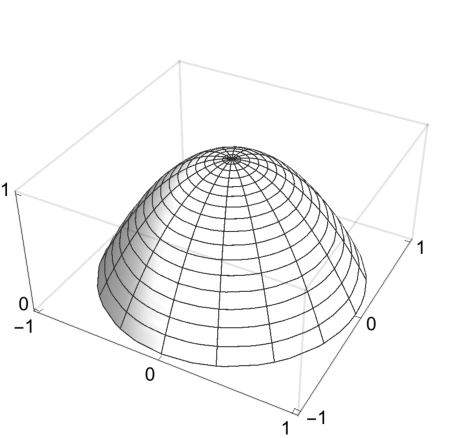
\includegraphics [ width = 1.25in ] {graphics/ucone_2}}   \\
		  %
		   $3$ && 
			 \raisebox{-0.5\height}{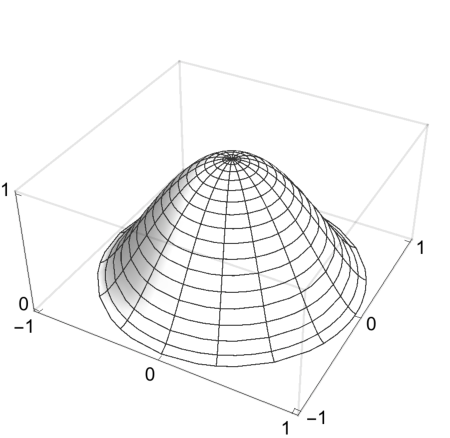
\includegraphics [ width = 1.25in ] {graphics/usphere_3}} &&
		   \raisebox{-0.5\height}{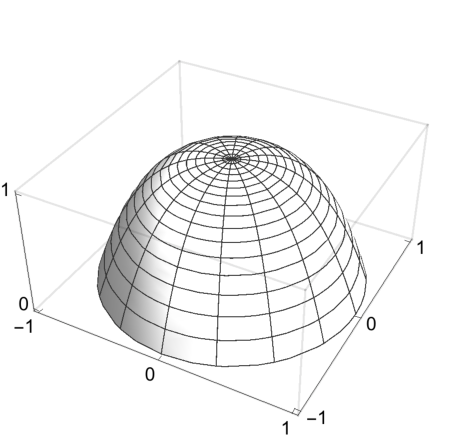
\includegraphics [ width = 1.25in ] {graphics/ucone_3}}   
		  %
		\end{tabular}
	\end{center}
\label{tab:progression}
\end{table}%

The analysis in the previous section broadens to the ultra families. If we extend \eqref{eq:rhov} to the following
% = =  e q u a t i o n
  \begin{equation}
    \begin{split}
     A\paren{\mu,\rho} & = 1 - \paren{\frac{1+\rho}{2}}^{\mu/2}, \\
     B\paren{\mu,\rho} & = \paren{\frac{1-\rho}{2}}^{\mu/2},
    \label{eq:end}    
    \end{split}
    %\label{eqn:}
  \end{equation}
% = = 
then
% = =  e q u a t i o n
  \begin{equation}
    \begin{split}
      \alpha\paren{\rho} &= - \paren{\frac{1+\rho} {2}}^{\mu/2}, \\
      \beta \paren{\rho} &=   \paren{\frac{1-\rho} {2}}^{\mu/2},
    \end{split}
  \end{equation}
% = =
and the parity relation in \eqref{eq:parity} holds. We can take $-\frac{1}{2}<\mu<\infty$ because the Legendre polynomials are complete on $L^{2}[-1,1]$ and both $A\paren{\mu,r}$ and $B\paren{\mu,r}$ are $L^{2}$ functions for this interval of the parameter $\mu$ for the domain of $r$. We must restrict the values of the parameter to $0<\mu<\infty$ because (a) we don't want to motivate infinities and (b) to preserve the fixed points at the center $\paren{A\paren{\mu,0} = B\paren{\mu,0}= 1}$, and  at the rim $\paren{A\paren{\mu,1} = B\paren{\mu,1}= 0}$.


%   ++   ++   ++   ++   ++   ++   ++   ++   ++   ++   ++   ++   ++   ++   ++   ++   ++   ++   ++   ++   ++   ++   ++   ++ 
\subsection{Integral equalities}
The previously cited work \cite[eq. 19]{22358} presents an integral expression for the equivalence of the cone and the sphere:
% = =  e q u a t i o n
  \begin{equation}
    %\begin{split}
      \int_{0}^{1} \paren{1-r} R_{n}^{0}(r) r dr = \paren{-1}^{n/2} \int_{0}^{1} \sqrt{ 1 - r^{2} }R_{n}^{0}(r) r dr, \quad n=0,2,4,\dots
    %\end{split}
    %\label{eqn:}
  \end{equation}
% = =
which can be reduced with the realization that Zernike polynomials for $n\ge1$ have zero mean:
% = =  e q u a t i o n
  \begin{equation}
    %\begin{split}
      \int_{0}^{1} \paren{1-r} R_{n}^{0}(r) r dr = - \int_{0}^{1} R_{n}^{0}(r) r^{2} dr, \quad n=2,4,\dots
    %\end{split}
    %\label{eqn:}
  \end{equation}
% = =
Unexpectedly, the integral equality extends to the ultra surfaces:
% = =  e q u a t i o n
\begin{equation}
  %\begin{split}
    \int_{0}^{1} \paren{1-r^{\mu}} R_{2k}^{0}(r) r dr = \paren{-1}^{k+1} \int_{0}^{1} \paren{ 1 - r^{2} }^{\mu/2}R_{2k}^{0}(r) r dr, \quad k=1,2,\dots
    \label{eq:integrals}
  %\end{split}
\end{equation}
% = =
where $\mu > -2$.

Sample equalities for three values of $\mu$ are shown in table \ref{tab:integrals}. The Zernike polynomial in each case is $R_{100}^{0}(r)$, displayed in figure \ref{fig:r100}.
\begin{figure}[htbp] %  figure placement: here, top, bottom, or page
   \centering
   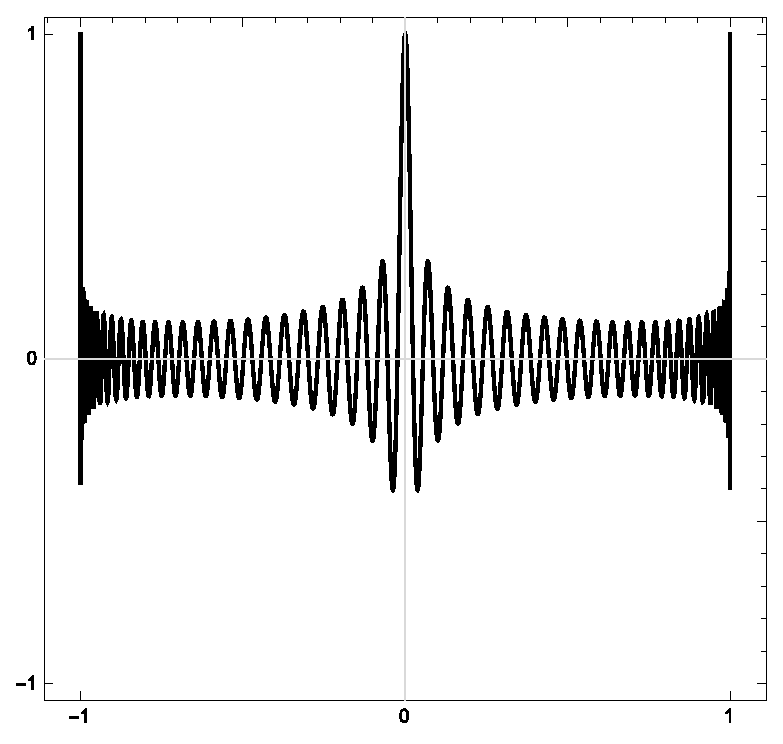
\includegraphics[ width = 2.5in ]{graphics/zernike_100_000} 
   \caption{The highly oscillatory polynomial $R_{100}^{0}(r)$. The period of oscillation shortens as $r$ increases; the first derivative at the boundary are growing rapidly. The radial polynomials are monic and the plot shows the function achieving unit value at $\abs{r}=1$; the displayed function also achieves unit value at $r=0$.}
   \label{fig:r100}
\end{figure}

\begin{table}[htbp]
\caption{Integral equalities in \eqref{eq:integrals} visualized for three different values of $\mu$. The integrands of interest are shown atop each column representing the ultra--surface, the Zernike polynomial $R_{100}^{0}(r)$ and the geometric factor $r$ from integrating over the unit disk. For constant $\mu$ (within each row), the area under each curve is the same.}
  \begin{center}
    \begin{tabular}{ccccc}
      %
      $\mu$ && ultra--cone && ultra--sphere \\\hline
      && \\
      %
      && $r \paren{1-r^{\mu}} R_{100}^{0}(r) $ && $r \paren{ 1 - r^{2} }^{\mu/2}R_{100}^{0}(r)$ \\[20pt]
      %
      $\frac{1}{4}$ &&
		   \raisebox{-0.5\height}{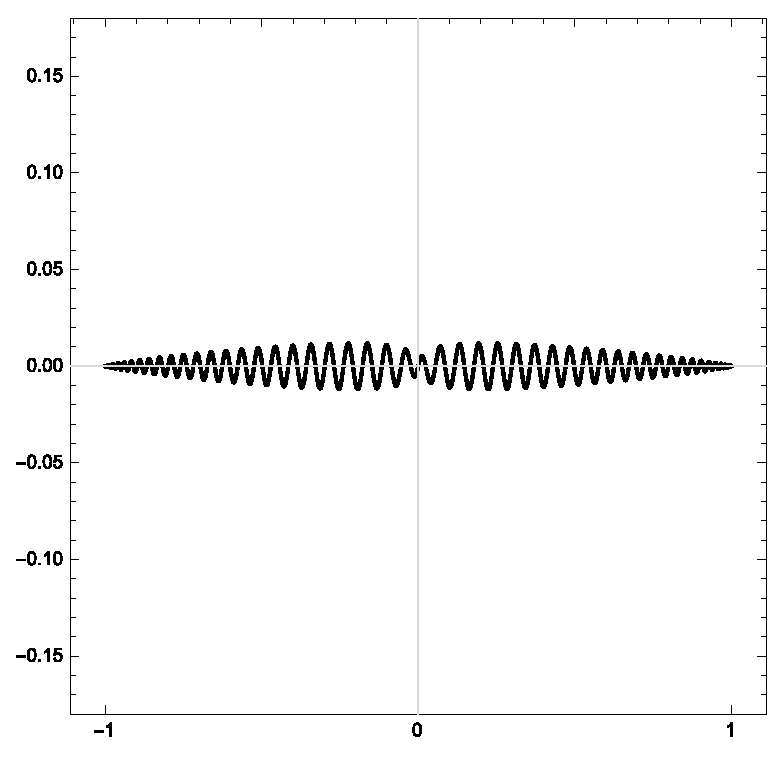
\includegraphics [ width = 1.75in ] {graphics/product_cone_025}} && 
		   \raisebox{-0.5\height}{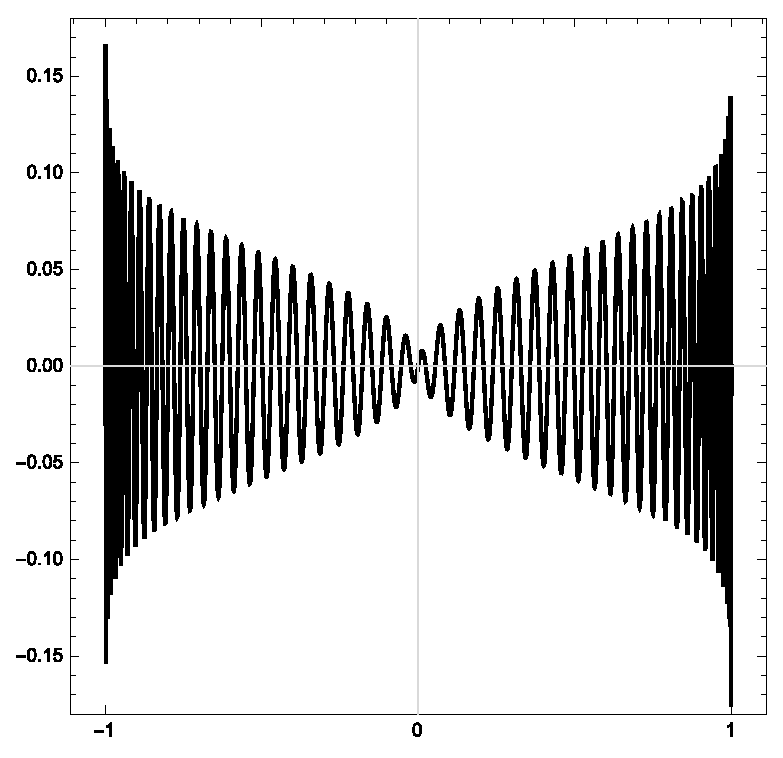
\includegraphics [ width = 1.75in ] {graphics/product_sphere_025}}   \\[70pt]      
      %
      1 &&
		   \raisebox{-0.5\height}{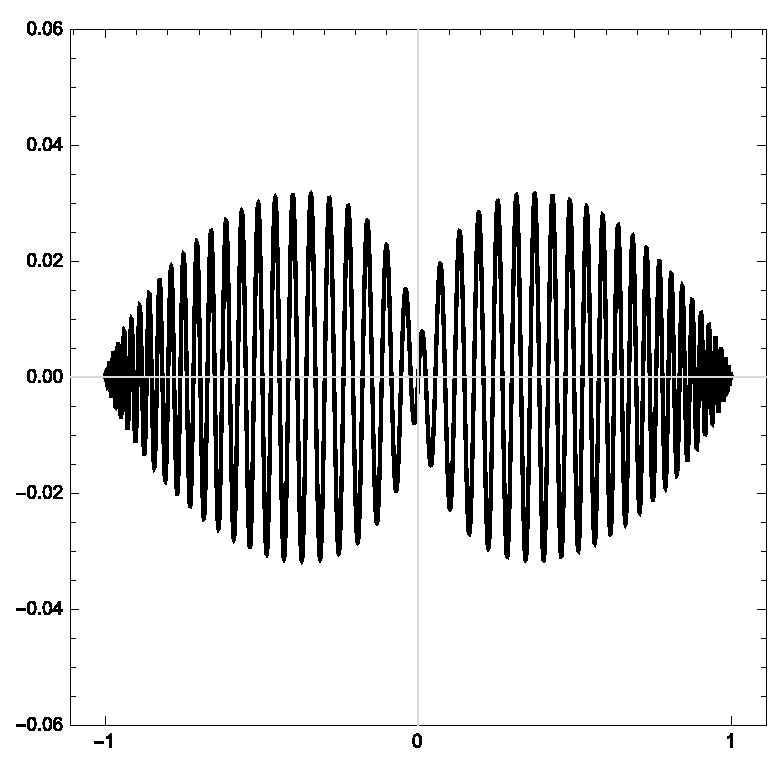
\includegraphics [ width = 1.75in ] {graphics/product_cone_1}} &&
		   \raisebox{-0.5\height}{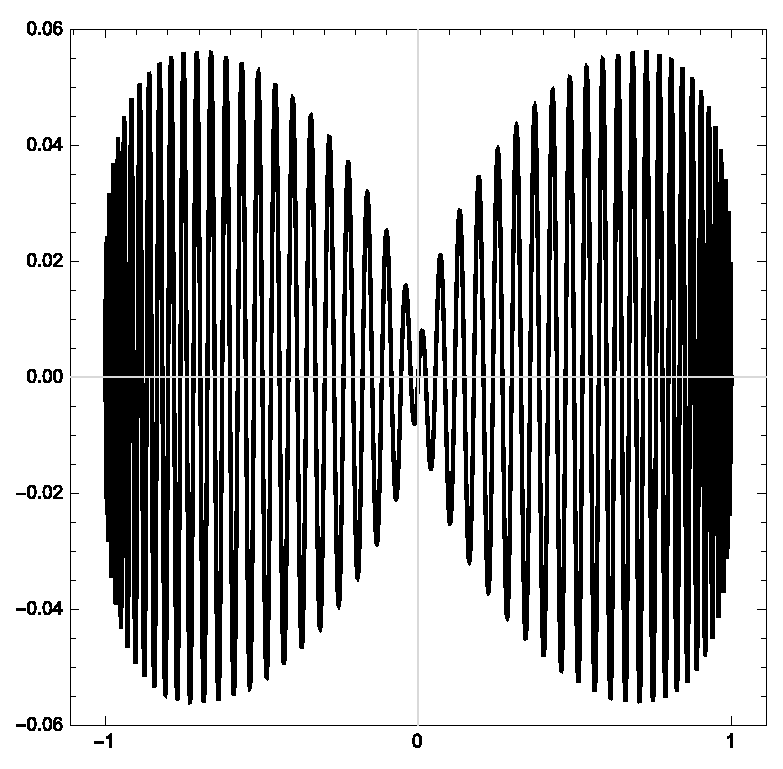
\includegraphics [ width = 1.75in ] {graphics/product_sphere_1}}   \\[70pt] 
      %
      9 &&
		   \raisebox{-0.5\height}{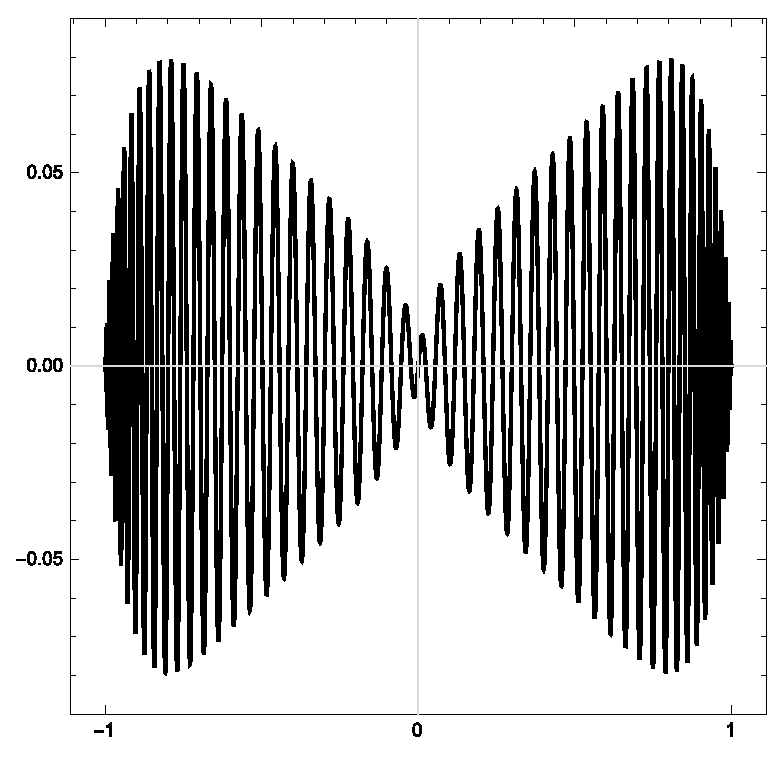
\includegraphics [ width = 1.75in ] {graphics/product_cone_9}} &&
		   \raisebox{-0.5\height}{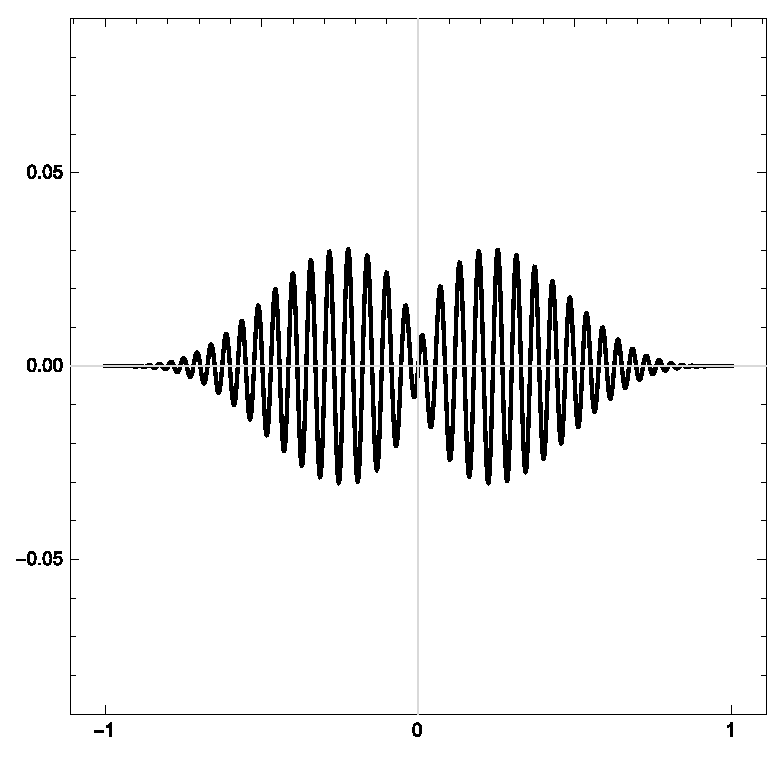
\includegraphics [ width = 1.75in ] {graphics/product_sphere_9}}      
      %
      %
    \end{tabular}
  \end{center}
\label{tab:integrals}
\end{table}%

%   +   +   +   +   +   +   +   +   +   +   +   +   +   +   +   +   +   +   +   +   +   +   +   +   +   +   +   +   +   +
\section{Discussion}
\label{sec:discussion}

The special cases for integer values of $\mu$ are interesting. When $\mu$ is an even integer the pathologies in both families disappear;  the ultra--cone has a polynomial representation $1-r^{\mu}$, as does the ultra--sphere  $\paren{1-r^{2}}^{\mu/2}$. The degenerate case for $\mu=2$ is a parabola which connects the ultra--cone and the ultra--sphere:
%
\begin{equation}
    A(2,r) = B(2,r) = 1 - r^{2}.
\end{equation}
%
When $\mu$ is an odd integer the pathologies move to the $\mu$th derivative. For the ultra--cone the jump in the $\mu$th derivative is $2\paren{\mu!}$. For the ultra--sphere the $\mu$th derivative is dominated by a term like $\paren{\frac{r} {\sqrt{1-r^{2}}}}^{\mu}$ near the boundary.

To summarize, when $\mu=2$ the two families produce the same surface. For all other values of $0<\mu<\infty$,
equations \eqref{eq:canona} and \eqref{eq:canonb} hold and the surfaces have equivalent regularity, $A\paren{\mu,r} \equiv B\paren{\mu,r}$. When $\mu$ is an odd number the surfaces have the recognized pathologies in the $\mu$th derivative.

%   ++   ++   ++   ++   ++   ++   ++   ++   ++   ++   ++   ++   ++   ++   ++   ++   ++   ++   ++   ++   ++   ++   ++   ++ 
\subsection{Regularity}
For the cone and the sphere $(\mu=1)$ we can exactly state the decay rate of the amplitudes shown in \eqref{eqn:archeoamps}: 
% = =  e q u a t i o n
  \begin{equation}
    \begin{split}
      \abs{a_{2k}} = \abs{b_{2k}} = \paren{ (2k - 1 ) ( 2k + 3 ) }^{-1}, \quad k = 1, 2, \dots
    \end{split}
    %\label{eqn:}
  \end{equation}
% = =
The cases for arbitrary $\mu$ are discussed below. While the Fourier-Zernike coefficients are defined as
% = =  e q u a t i o n
\begin{equation}
  %\begin{split}
    a_{2k}\paren{\mu} = 2\paren{2k+1} \int_{0}^{1} \paren{1 - r}^{\mu} R_{2k}^{0}(r) r dr, \qquad k=0,1,2,\dots
    %\label{eqn:}
  %\end{split}
\end{equation}
% = =
a simpler form is available. The first term $\paren{k=0}$ is given by
% = =  e q u a t i o n
\begin{equation}
  \begin{split}
      a_{0}(\mu) &=  \frac{2}{\mu + 2},
    %\label{eqn:}
  \end{split}
\end{equation}
% = =
subsequent terms $\paren{k\ge1}$ are
% = =  e q u a t i o n
\begin{equation}
  %\begin{split}
    a_{2k}(\mu) = \paren{-1}^{k} 2\paren{2k+1} \prod_{j=0}^{k-1}\paren{\mu - 2j} \paren{\prod_{j=0}^{k}\paren{\mu + 2(j+1)}}^{-1}
    %\label{eqn:}
  %\end{split}
\end{equation}
% = =
which holds for $\mu>-2$. The recursion relationship for jumping from $2k$ to $2k+2$ is given by
% = =  e q u a t i o n
  \begin{equation}
    %\begin{split}
      a_{2k+2} = - a_{2k} \frac{2k+1} {2k-1} \frac{\mu - 2(k-1)} {\mu + 2\paren{k + 2}}, \qquad k = 1,2,3, \dots
    %\end{split}
    %\label{eqn:}
  \end{equation}
% = =

The increasing rapidity of decay for the expansion amplitudes and onset of asymptotic form for the higher order pathological surfaces is shown in figure \ref{fig:mu big}. The surfaces where $\mu$ is even have polynomial form with $1+\mu/2$ nonzero amplitudes.

\begin{figure}[htbp] %  figure placement: here, top, bottom, or page
   \centering
%   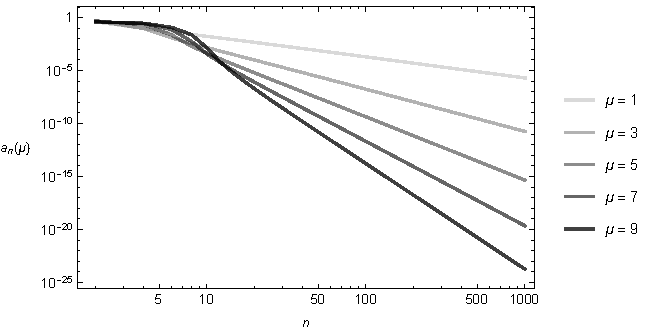
\includegraphics[ width = 5in ]{graphics/decay_big} 
   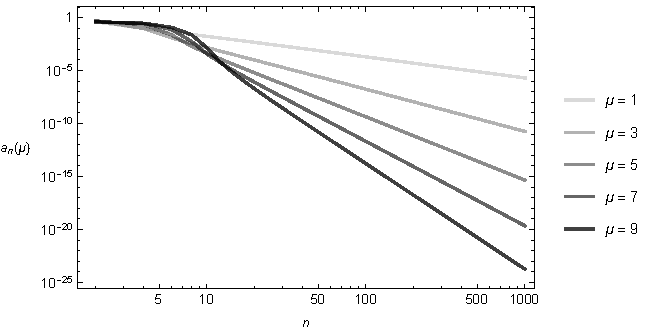
\includegraphics[ width = 5in ]{graphics/decay_big} 
   \caption{Absolute value of the expansion amplitudes for the ultra surfaces with $\mu$ increasing arithmetically from unity through the odd numbers. The ultra--cone has a jump in the $\mu$th derivative at $r=0$. The $\mu$th derivative of the ultra--sphere is unbounded at $r=1$. }
   \label{fig:mu big}
\end{figure}

\begin{figure}[htbp] %  figure placement: here, top, bottom, or page
   \centering
%   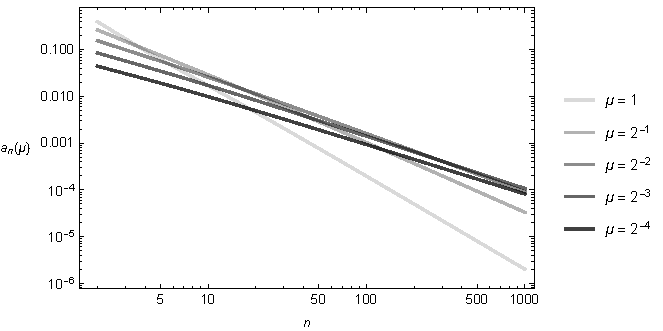
\includegraphics[ width = 5in ]{graphics/decay_small} 
   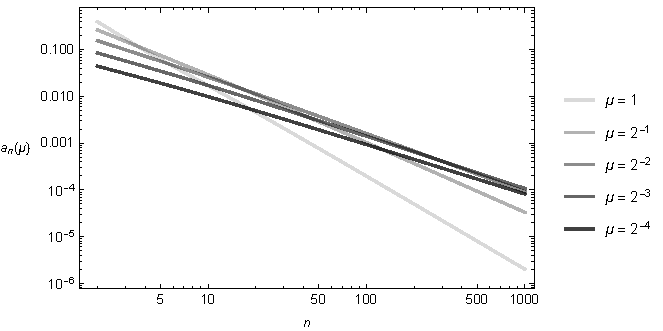
\includegraphics[ width = 5in ]{graphics/decay_small} 
   \caption{Absolute value of the expansion amplitudes for the ultra surfaces with $\mu$ decreasing in a geometric series. First derivative pathologies persist in the continuum of values $-2<\mu\le1$.}
   \label{fig:mu small}
\end{figure}

%   ++   ++   ++   ++   ++   ++   ++   ++   ++   ++   ++   ++   ++   ++   ++   ++   ++   ++   ++   ++   ++   ++   ++   ++ 
\subsection{Homotopies}
The ultra--cone and the ultra--sphere each represent a homotopy family. The transformation which deforms the cone state $\mu_{1}$ to the state $\mu_{2}$ is
% = =  e q u a t i o n
  \begin{equation}
    %\begin{split}
      f\paren{\mu_{1}, \mu_{2},r} = \frac{A\paren{\mu_{2},r}} {A\paren{\mu_{1},r}} = \frac{1-r^{\mu_{2}}} {1-r^{\mu_{1}}},
    %\end{split}
    %\label{eqn:}
  \end{equation}
% = = 
and the transformation which deforms the sphere state $\mu_{1}$ to the state $\mu_{2}$ is
% = =  e q u a t i o n
  \begin{equation}
    %\begin{split}
      g\paren{\mu_{1}, \mu_{2},r} = \frac{B\paren{\mu_{2},r}} {B\paren{\mu_{1},r}}  = \paren{\sqrt{1-r^{2}}}^{\mu_{2} - \mu_{1}}.
    %\end{split}
    %\label{eqn:}
  \end{equation}
% = =

These two distinct homotopy families are related through the special case of $\mu=2$ which merges the ultra--cone with the ultra--sphere. For example to go from cone state $A\paren{\mu_{1},r}$ to sphere state $B\paren{\mu_{2},r}$ the deformation is
\begin{equation}
  B\paren{\mu_{2},r} = f\paren{\mu_{1}, 2,r} g\paren{2, \mu_{2},r} A\paren{\mu_{1},r}.
\end{equation}
The fixed points for these transformations are the origin $r=0$ and the perimeter $r = 1$.

%   +   +   +   +   +   +   +   +   +   +   +   +   +   +   +   +   +   +   +   +   +   +   +   +   +   +   +   +   +   +
\section{Conclusion}
\label{sec:conclusion}
By extending tools of Fourier analysis we have discovered an intriguing equivalence between the cone and the sphere in the basis of the rotationally invariant $(m=0)$ Zernike polynomials. Both of these surfaces are pathological in the first derivative; the cone at the apex, the sphere at the boundary. Such an equivalence led to the discovery of the ultra surfaces and inspired a formal evaluation of these homotopy families connecting the sphere and the cone.

The author P.F.E thanks Los Alamos National Laboratory (LANL) for support during the summer of 2010. This report will be available in the LANL archives as LA-UR-mmmmm.

%% The Appendices part is started with the command \appendix;
%% appendix sections are then done as normal sections
%% \appendix

%% \section{}
%% \label{}

%% If you have bibdatabase file and want bibtex to generate the
%% bibitems, please use
%%
%%  \bibliographystyle{elsarticle-num} 
%%  \bibliography{<your bibdatabase>}

%% else use the following coding to input the bibitems directly in the
%% TeX file.

\begin{thebibliography}{00}

%% \bibitem{label}
%% Text of bibliographic item

\bibitem{BW} M. Born and E. Wolf.
\newblock  {\em Principles of Optics : Electromagnetic Theory of Propagation, Interference and Diffraction of Light,} 7e.
\newblock  Cambridge University Press, 1999.
  
\bibitem{Hecht} M.S. Hecht.
\newblock  {\em Optics,} 4e.
\newblock  Addison Wesley, 2001.

\bibitem{do} O. Marchenko, S.~A. Kazantsev, and L. Windholz.
\newblock  {\em Demonstrational Optics: Wave and geometrical optics,} 3e.
\newblock  Springer, 2003.

\bibitem{Longair} M.S. Longair.
\newblock  {\em High Energy Astrophysics,} 3e.
\newblock  Cambridge University Press, 2011.

\bibitem{Green} D. Green.
\newblock  {\em The Physics of Particle Detectors,} 
\newblock  Cambridge University Press, 2005.

\bibitem{22358} D. Topa, J. Cooley and P. Embid.
\newblock  {\em Which is smoother: the sphere or the cone?}
\newblock  LANL report LA-UR-22358, 2012.

\bibitem{classic} L. Grafakos.
\newblock  {\em Classical Fourier Analysis,} 2e
\newblock  Springer, 2008.

\bibitem{modern} L. Grafakos.
\newblock  {\em Modern Fourier Analysis,} 2e
\newblock  Springer, 2009.

\bibitem{Simon} B. Simon.
\newblock  {\em Orthogonal Polynomials on the Unit Circle: Part 1: Classical Theory; Part 2: Spectral Theory,}
\newblock  American Mathematical Society, 1999.

\bibitem{Kanjin}
Y.~Kanjin, Banach Algebra Related to Disk Polynomials, 
\emph{T\^ohoku Math. J.}, vol.~37, pp. 395--404, 1985.

\bibitem{Zernike}
F. Zernike, Diffraction theory of the knife-edge test and its improved form, the phase-contrast method, 
\emph{Mon. Not. R. Astron. Soc.}, vol.~94, pp. 377--384, 1934.

\bibitem{Wolf}
A.~B. Bhatia, and E. Wolf, On the circle polynomials of Zernike and related orthogonal sets, 
\emph{Math. Proc. Cam. Phil. Soc.}, vol.~50, pp. 40--48, 1950.

\bibitem{Lax} P. Lax.
\newblock  {\em Functional Analysis,}
\newblock  Wiley, 2002.

\bibitem{Siegal}
A.R. Siegal, On the \mst theorem for $C[0,1]$, 
\emph{Proc. Amer. Math. Soc.}, vol.~36, pp. 161--166, 1972.

\bibitem{ms}
T. Trent, A \mst theorem for $C\paren{\overline{D}}$, 
\emph{Proc. Amer. Math. Soc.}, vol.~83, pp. 296--298, 1981.

\end{thebibliography}
\end{document}
\endinput

% Daniel Topa
% dantopa@gmail.com
% 505 504 5986
%%
%% End of file `elsarticle-template-num.tex'.
